\documentclass[bibliography=totocnumbered,a4paper,10pt]{scrartcl}
\usepackage[utf8]{inputenc}
\usepackage{amsmath,amsthm, amssymb, latexsym}
\usepackage{epstopdf,graphicx,hyperref}
\usepackage{listings,xcolor,float,multirow}
\usepackage{array}
\usepackage{longtable}
\usepackage[a4paper, total={6in, 9in}]{geometry}
\usepackage{xspace}

%==============%
%  Code Style  %
%==============%
\definecolor{gray}{rgb}{0.5,0.5,0.5}
\lstset{
  basicstyle=\ttfamily,
  commentstyle=\color{gray}\ttfamily,
  columns=fullflexible,
  language=bash, 
  frame=l,
  showstringspaces=false
}

%==============%
%  References  %
%==============%
\usepackage[backend=biber,
            sorting=none,
            style=chem-acs]{biblatex}
\addbibresource{SerenityUserManual.bib}
\renewcommand{\cite}[1]{\supercite{#1}}
%==========%
%  Macros  %
%==========%

\makeatletter
\def\ifemptyarg#1{%
  \if\relax\detokenize{#1}\relax %
    \expandafter\@firstoftwo
  \else
    \expandafter\@secondoftwo
  \fi}
\makeatother

\newcommand{
\serenity}{\textsc{Serenity}\xspace}

\definecolor{expert}{HTML}{7D0C0C}

%
% Normal Keyword
%
\newcommand\nkeyword[4]{\parbox[c]{3.5cm}{\vspace{.3\baselineskip} \centering #1 \vspace{.3\baselineskip}} & 
                        \parbox[c]{3cm}{\vspace{.3\baselineskip}\centering #2 \vspace{.3\baselineskip}} & 
                        \parbox[c]{8cm}{\vspace{.3\baselineskip}\textit{#3}\ifemptyarg{#4}{}{\\#4}\vspace{.3\baselineskip}}\\ \hline}
%
% Expert Keyword
%
\newcommand\ekeyword[4]{
                        \parbox[c]{3.5cm}{\vspace{.3\baselineskip} \centering \color{expert}{#1} \vspace{.3\baselineskip}} & 
                        \parbox[c]{3cm}{\vspace{.3\baselineskip}\centering\color{expert}{#2}\vspace{.3\baselineskip}} & 
                        \parbox[c]{8cm}{\vspace{.3\baselineskip}\color{expert}{\textit{#3}\ifemptyarg{#4}{}{\\#4}}\vspace{.3\baselineskip}}\\ \hline}
%
% Headder
%
\newcommand\headder{\parbox[c]{3.5cm}{\vspace{.3\baselineskip} \centering Keyword \vspace{.3\baselineskip}} & 
                       \parbox[c]{3cm}{\vspace{.3\baselineskip} \centering \textit{Type} or VALUES [Default] \vspace{.3\baselineskip}} & 
                       \parbox[c]{8cm}{\vspace{.3\baselineskip} \centering \textit{Keyword Description} \& Options Descriptions \vspace{.3\baselineskip} }\\ \hline}

\newcommand{\taskoptions}[5]{
\begin{longtable}{|>{\ttfamily}c|>{\ttfamily}c|l|} \hline
    \multicolumn{3}{|c|}{\parbox[c]{14.5cm}{\centering\vspace{.3\baselineskip}\textbf{Standard Keywords}\vspace{.3\baselineskip}}} \\ \hline
    \parbox[c]{3.5cm}{\centering\vspace{.3\baselineskip}Task Name\vspace{.3\baselineskip}} 
      & \multicolumn{2}{l|}{\parbox[c]{11cm}{\vspace{.3\baselineskip}\texttt{#1}\vspace{.3\baselineskip}}} \\ \hline 
    \parbox[c]{3.5cm}{\centering\vspace{.3\baselineskip}Active Systems\vspace{.3\baselineskip}} 
      & \multicolumn{2}{l|}{\parbox[c]{11cm}{\vspace{.3\baselineskip}#2\vspace{.3\baselineskip}}}          \\ \hline
    \parbox[c]{3.5cm}{\centering\vspace{.3\baselineskip}Environment Systems\vspace{.3\baselineskip}} 
      & \multicolumn{2}{l|}{\parbox[c]{11cm}{\vspace{.3\baselineskip}#3\vspace{.3\baselineskip}}}   \\ \hline
    \parbox[c]{3.5cm}{\centering\vspace{.3\baselineskip}Possible Blocks\vspace{.3\baselineskip}} 
      & \multicolumn{2}{l|}{\parbox[c]{11cm}{\vspace{.3\baselineskip}#4\vspace{.3\baselineskip}}}   \\ \hline \hline
    \multicolumn{3}{|c|}{\parbox[c]{14.5cm}{\centering\vspace{.3\baselineskip}\textbf{Specific Keywords}\vspace{.3\baselineskip}}} \\ \hline 
    \parbox[c]{3.5cm}{\vspace{.3\baselineskip} \centering Keyword \vspace{.3\baselineskip}} & 
                       \parbox[c]{3cm}{\vspace{.3\baselineskip} \centering \textit{Type} or VALUES [Default] \vspace{.3\baselineskip}} & 
                       \parbox[c]{8cm}{\vspace{.3\baselineskip} \centering \textit{Keyword Description} \& Options Descriptions \vspace{.3\baselineskip} }\\ \hline
    #5
\end{longtable} 
}

%============%
%  Document  %
%============%
\begin{document}
\thispagestyle{empty}
\begin{center}
\vspace*{1cm}

\includegraphics[width=0.95\textwidth]{./figs/SerenityLogo.png}\\
%{\Huge
% \textsc{Serenity}
%}\\
\vspace{2cm}
{\LARGE\textbf{
User Manual
}}\\
\vspace{1cm}
{\large\textbf{
Program Version: 1.2.0\\
Manual Generated: \today
}}\\
\vspace{2cm}
{\large\textbf{ 
The Serenity Developers$^{\dagger}$\footnote{Release Repository: \texttt{http://guthub.com/qcserenity/serenity}\\
                                             Developer Repository: \texttt{http://thclab.uni-muenster.de/serenity/serenity}}
\footnote{For questions and requests pertaining the manual please contact:\\ \texttt{serenity@uni-muenster.de}}
}}\\
\vspace{2cm}
{\large Manual edited by: \\
Jan P.\ Unsleber
}
\\[2ex]

$^{\dagger}$ Theoretische Organische Chemie,
Organisch-Chemisches Institut \\
and Center for Multiscale Theory and Computation,\\
Westf\"alische Wilhelms-Universit\"at M\"unster\\
Corrensstra{\ss}e 40, 48149 M\"unster, Germany\\[2ex]

\vfill
\end{center}
\newpage
\pagenumbering{Roman}
\setcounter{page}{1}
\tableofcontents

\newpage
\pagenumbering{arabic}
\setcounter{page}{1}
\numberwithin{equation}{subsubsection}
\section{Preface}
Subsystem and quantum embedding approaches are currently among the most quickly developing
methods in quantum chemistry. This is mostly due to their computational efficiency
and their easy interpretability in terms of intuitive, well-defined chemical subunits.
While the general idea of combining electronic-structure methods of different or the same
types for separate fragments is maybe straightforward, the practical execution of such
calculations can be a frustrating experience. The background is that such a combination
may require interfacing of different codes with limited interoperability through text files.
This strategy can be very successful, but usually also causes an overhead of work for the specific
interfaces needed. Moreover, it is vulnerable to (even slight) changes in the input/output
structure or working principles of the original programs. Even if all technical challenges
are dealt with, inexperienced users may find it hard to choose the optimum embedding approach
for a problem at hand, since comparison of different schemes can be very difficult.\\
\\
This was our motivation for developing a new quantum chemistry code that should give access
to a wide variety of quantum embedding approaches. This should allow for easy comparisons
of embedding schemes, as \serenity is written with a subsystem structure in mind right from
the beginning. Hence, it includes several possibilities for embedding calculations with
different ingredients. Its modular structure should make it easily extensible to upcoming
embedding features. As an open-source project, it may be tailored to user-specific requirements
whenever desired.\\
\\
The following manual shows how to use \serenity as a standalone program. Its usage as a
library is best explained through the source code (detailed manual 
information may follow at a later point).



\newpage
\section{Install}
Please read the following instructions carefully, these instructions can also be found in the \texttt{README.md} distributed with
the source code.

\subsection{Prerequisites}

The code has been tested and compiled with GCC/G++ (Versions 4.X, 5.X, 6.X and 7.X)
and ICC/ICPC (Versions 17.X) compilation with other compilers and versions might still
be possible though.\\

The compilation of the code is supported on Linux systems, and should be possible on MacOS
the latter however is still to be tested thoroughly.\\

In order to allow for the correct installation of Serenity unsing the source code, 
the compilation process will need to download the pre-configured version of Libint hosted 
in the ext-libint project on thclab.uni-muenster.de.
Libint will be downloaded using an SSH connection, to this end please make sure that
a public SSH key is added to your profile on the GitLab server.\\

The following programs/libraries must be available on your system:
\begin{itemize}
 \item CMake (Version >= 3.9)
 \item Boost (for package managers: including boost-devel)
 \item OpenMP
 \item Eigen3 
 \item HDF5 (Version >= 1.10.1; including header files and cmake files)
 \item A recent GMP version, including C++ support (for libint2)
 \item The standard GNU toolchain (make, tar, autoconf, libtool)  
\end{itemize} 
The following libraries may be preinstalled and will otherwise be automatically 
downloaded and installed locally:
\begin{itemize}
 \item xcfun (The Serenity verison is forked to: https://github.com/moritzBens/xcfun.git)  
 \item libecpint (The Serenity version is forked to: https://github.com/moritzBens/libecpint.git)  
\end{itemize} 
The following libraries will be downloaded and installed locally regardless of their earlier
presence:
\begin{itemize}
 \item GTest (Google Test and Google Mock)
 \item libint2 (Version 2.2.0-beta3, pre-configured and hosted at: https://thclab.uni-muenster.de/serenity/ext-libint)
\end{itemize} 
The following libraries are optional and needed for additional features:
\begin{itemize}
 \item Intel MKL (for SMP parallel Eigen3 eigenvalue solvers)
 \item Doxygen (for the documentation)
 \item Python-devel (for the python wrapper)   
 \item pybind11 (for the python wrapper)
\end{itemize} 

\subsection{Install Using CMake and Make}

Extract or pull the source code, then create a build directory:
\begin{lstlisting}
cd serenity
mkdir build  
cd build  
\end{lstlisting}
Then run cmake:
\begin{lstlisting}
cmake ..    
\end{lstlisting}
(If the build folder is not located inside the main directory of \textsc{Serenity}
please adapt the path accordingly.)

Finally run make and make install to build the program:
\begin{lstlisting}
make         
\end{lstlisting}
Please source serenity.sh located in the main folder to set all necessary environment 
variables:
\begin{lstlisting}
cd ..  
source serenity.sh
\end{lstlisting}
\subsection{Install Including Python Interface}
In order to activate the compilation of a Python interface to the code
a flag can be set as follows
\begin{lstlisting}
cmake -DSERENITY_PYTHON_BINDINGS=ON ..
\end{lstlisting}
additionally this and other flags can be toggled using `ccmake`
\begin{lstlisting}
ccmake ..
\end{lstlisting}
The wrapper will be build for the Python version that CMake finds first
In order to point CMake to a specific version of Python the following 
option can be used:
\begin{lstlisting}
cmake -DPYTHON_EXECUTABLE=/usr/bin/python3 ..
\end{lstlisting}
The wrapper is shipped in form of a shared library (serenipy.so).
In order for Python to find this package the library folder has to be present 
in the \texttt{PYTHONPATH} environment variable and the Serenity library has to be 
present in a path searchd by the system for shared libraries.
The latter is done when sourceing the \texttt{serenith.sh} script, the former requires 
to uncomment one line in this file.
Afterwards the interface should importable as follows:
\begin{lstlisting}
python3
import serenipy as spy  
\end{lstlisting}
\subsection{Tests}
Serenity comes with a decent set of unittests in order to run them source 
the \texttt{serenity.sh} script and run
\begin{lstlisting}
PATH_TO_BUILD_DIR/bin/serenity_tests
\end{lstlisting}
Please use the complete path, or else GTEST might run into problems.  
  
The Python wrapper comes with its own set of tests, these can be run using
\begin{lstlisting}
python -m unittest discover PATH_TO_SERENITY/src/python/tests
\end{lstlisting}
\subsection{Documentation}
After configuring the project using CMake it is possible to create the documentation 
using:
\begin{lstlisting}
make doc
\end{lstlisting}
Then you can open up the doc/html/index.html in a browser.  
The python wrapper is not featured inside the documentation.
Its documentation is available via pythons help() function,
which displays the build-in doc-strings.

\clearpage
\section{Text Input}

The input of \serenity has two main types of sections, the \texttt{system} blocks and the \texttt{task} blocks.
A chart depicting how \serenity handles input can be seen in Figure~\ref{fig:input}. 
While the chart is already quite technical, it displays how to read the sectioned input.
Starting from the right, the main job of the program is to run tasks in a certain order.
These tasks can be related \textit{via} the systems they use, \textit{i.e.} a \texttt{MP2Task} will used
orbital data from a previous \texttt{SCFTask} if both of them are working with the same system.
Accordingly the input first needs a set of definitions for all the systems in this run, and then
a list of tasks to complete with these systems.
Here the systems are in a minimal case just a geometry and a set of settings (such as charge, spin, basis set, and so on).
During the run these systems will be populated with more (calculated) data, such as orbitals, energies and electron densities.
This additional data can also be read from previous runs (see the following section).
Any feature that \serenity has is implemented as a task (or a part of a task).
For a list of available features/tasks, see Section~\ref{sec:tasks}.
\begin{figure}[h!]
\label{fig:input}
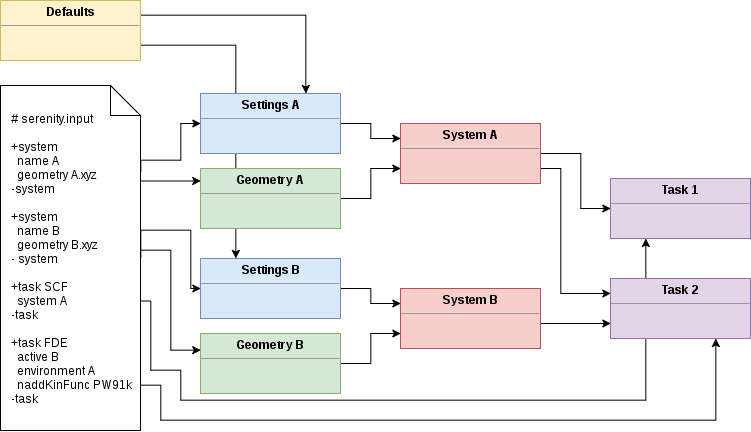
\includegraphics[width=0.95\textwidth]{./figs/SerenityInput.png}
\caption{Input flow of \serenity.}
\end{figure}\\
As stated above, the text input of \serenity is structured into blocks, and each block then contains keywords.
A keyword consists of a name and a value and is always given inside of a block. 
Each keyword-value pair has to be given in one separate line. 
As for the blocks, there are two main types, those are \texttt{system} and \texttt{task}. 
A block in the {\serenity} text input is started by a \texttt{+<blockname>} and ended with a
\texttt{-<blockname>}.
The \texttt{system} block can have one layer of sub-blocks, other than that, there is no further nesting
of blocks.\\
The the main blocks of a simple input might thus look like this:
\begin{lstlisting}
+system
 name water
 xyz ./water.xyz
 method dft
 +dft
  functional PBE
 -dft
-system

+task scf
  system water
-task
\end{lstlisting}
While there are many settings and thus many keywords, all of them are defaulted, and
each run of the program will create a file containing all settings (even the default ones)
for restart purposes.\\
The input accepts comments just like shell scripts.
Thus everything preceded  by a hash is not parsed. 
This holds for entire lines but also for parts of a line.
\begin{lstlisting}
# not parsed
+system # also not parsed
 name test
 # you guessed it, this is also not parsed
-system
\end{lstlisting}
The entire input (with the exception of system names and path names) is case-insensitive.
Keywords could thus look like this:
\begin{lstlisting}
  gradients true
  funcTIONAL PbE0
  maxCycles 123
  NaMe water # note that the value of name is case sensitive
\end{lstlisting}
A list of values for a keyword can be parsed by enclosing them into curly brackets:
\begin{lstlisting}
  orbitals {1 2 3 4}
\end{lstlisting}
A list of settings (keywords) inside the \texttt{system} and \texttt{task} blocks will be 
presented in the following two sections.

\newpage
\subsection{Systems}\label{sec:system}
Each system is defined by one system block, a system block contains general keywords and can contain one layer of sub-blocks.
All relevant keywords are discussed in this section.
The values given in square brackets ``\texttt{[..]}" or marked with a ``\texttt{[d]}" are the defaults.
The keywords given in red are suggested only to be used by advanced/expert users.
\subsubsection{General Keywords}\label{sec:system:general}
The keywords given directly inside the system block and not within one of the nested blocks are presented
in this section.\\
A regular system will need both the \texttt{geometry} and also the \texttt{name} keyword.
Further keywords can be given if their values need to differ from the defaults.
A loaded system only needs the \texttt{load} keyword and a \texttt{name}.
All other keywords will be deduced from the stored settings.
\begin{table}[H]\small \centering  \begin{tabular}{|>{\ttfamily}c|>{\ttfamily}c|l|} \hline 
\headder
\nkeyword{name}    {\textit{str} [default]}{The name of the system.}{}
\nkeyword{geometry}{\textit{str}          }{The path to the geometry (.xyz)}{This or \texttt{load} has to be given.}
\nkeyword{path}    {\textit{str} [./]     }{The path to store HDF5 files.}{}
\nkeyword{load}    {\textit{str} [ ]      }{The path to load HDF5 files from.}{If this is given all other settings are read, and given ones replaced.}
\nkeyword{charge  }{\textit{int} [0]      }{The charge of the system.}{}
\nkeyword{spin    }{\textit{int} [0]      }{The spin of the system.}{Given as alpha spin electron excess.}
\nkeyword{scfmode }{RESTRICTED [d] \\UNRESTRICTED}{The orbital mode of the SCF.}{
Use closed shell calculations for this system (\texttt{RESTRICTED}), or use open shell calculations for this system (\texttt{UNRESTRICTED}).}
\nkeyword{method  }{HF [d] \\ DFT}{The general electronic structure method for this system.}{Generate Hartree-Fock orbitals, or generate DFT orbitals.}
\end{tabular}\end{table}


\newpage
\subsubsection{SCF Block}\label{sec:system:scf}
All settings available pertaining the SCF and its convergence are given in this sub-block of the system block.
\begin{table}[H]\small \centering \begin{tabular}{|>{\ttfamily}c|>{\ttfamily}c|l|} \hline 
\headder
\nkeyword{initialguess}{HCORE\\EHT\\ATOM\_DENS\\ATOM\_SCF [d]\\SAP}{The initial guess for the electronic structure.}{
$h_{core}$ guess, i.e. ignoring electron-electron interactions, or an
extended Hueckel theory (EHT) guess, or a guess of combined atomic densities (\texttt{ATOM\_DENS}).
\texttt{ATOM\_SCF} is similar to \texttt{ATOM\_DENS}, but the atomic densities 
themselves are calculated with a proper SCF for each atom type, furthermore a superposition of
atomic potentials (SAP) is available.}{}
\nkeyword{damping}{NONE\\SERIES [d]\\STATIC}{The mode of damping of the new Fock matrix with the last one during the SCF.}{
No damping (\texttt{NONE}), or a damping value decreasing in each step (\texttt{SERIES}), 
or a static damping value set by the \texttt{staticDampingFactor} keyword.}{}
\nkeyword{maxCycles          }{ \textit{ int} [100]     }{Maximum number of SCF cycles. }{} 
\nkeyword{writeRestart       }{ \textit{ int} [5]       }{Interval to write checkpoints during SCF. }{}
\nkeyword{energyThreshold    }{ \textit{ double} [1e-8] }{Convergence criterion for the energy.}{}
\nkeyword{rmsdThreshold      }{ \textit{ double} [1e-8] }{Convergence criterion for the density matrix.} {}
\nkeyword{diisThreshold      }{ \textit{ double} [1e-7] }{The convergence criterion for the DIIS ([F,P]) error. } {}
\nkeyword{densityFitting}{NONE\\RI [d]\\CHOLESKY}{Modes of fitting the density in 2e-4c-integrals.}{
No density fitting, full two electron four center evaluation $(n^4)$, or
Resolution of identity fitting (\texttt{RI}) for the Coulomb part $(n^3)$ (non-hybrid DFT only).
Cholesky decomposition for all four center integrals $(n^3)$, is NOT YET AVAILABLE!} 
\ekeyword{seriesDampingStart }{ \textit{ double} [0.7]   }{Start value for the series damping. } {}
\ekeyword{seriesDampingEnd   }{ \textit{ double} [0.6]   }{End value for the series damping. } {}
\ekeyword{seriesDampingStep  }{ \textit{ double} [0.05]  }{Increment value for the series damping. } {}
\ekeyword{seriesDamping\\InitialSteps}{ \textit{ int} [2]}{Number of initial steps without increment } {}
\ekeyword{staticDampingFactor}{ \textit{ double} [0.7]   }{Damping value for the static damping.}{} 
\ekeyword{diisStartError     }{ \textit{ double} [0.1]   }{[F,P] value at which the DIIS starts. } {}
\ekeyword{diisMaxStore       }{ \textit{ int} [5]        }{The number of Fock Matrices stored int the DIIS} {}
\ekeyword{diisCondition\\NumberThreshold}{\textit{double} [1000.0]}{Inverse SVD threshold for the DIIS.} {}
\end{tabular}\end{table}
\newpage
\subsubsection{Basis Block}\label{sec:system:basis}
All settings available pertaining the usage and generation of basis sets.
The basis sets can be found in \texttt{data/basis}. These are not exclusive. Any folder with \textsc{Turbomole}
style basis sets can be given and every file can be added to it, given that the file names are spelled in 
uppercase.
\begin{table}[H]\small \centering  \begin{tabular}{|>{\ttfamily}c|>{\ttfamily}c|l|} \hline 
\headder
\nkeyword{label             }{ \textit{ str} [6-31Gs]        }{Basis set name. }{}
\nkeyword{makeSphericalBasis}{ \textit{ bool} [false]        }{Use spherical harmonics basis (slow; not recommended). }{} 
\nkeyword{basisLibPath      }{ \textit{ str} [\$ENV]         }{Basis set file location (default taken from environment variable). }{} 
\nkeyword{auxJLabel         }{ \textit{ str} [RI\_J\_Weigend]}{Auxiliary basis set name for Coulomb interactions (RI). }{} 
\nkeyword{auxCJLabel        }{ \textit{ str} [auto]          }{Auxiliary basis set name for Correlation interactions (RI). }{}
\nkeyword{firstECP          }{ \textit{ int} [37]            }{Atomic number threshold for the use of ECPs if available in the basis set. }{}
\ekeyword{integralThreshold }{ \textit{ double} [1e-10s]     }{Threshold for the prescreening in integral evaluations.}{} 
\end{tabular}\end{table}

\subsubsection{Grid Block}\label{sec:system:grid}
All settings available to tune the generation of integration grids.
\begin{table}[H]\small \centering  \begin{tabular}{|>{\ttfamily}c|>{\ttfamily}c|l|} \hline 
\headder
\nkeyword{smallGridAccuracy     }{ \textit{int} [2]        }{Accuracy for intermediate grids.}{Range: 1-7, with 7 being most accurate.} 
\nkeyword{accuracy              }{ \textit{int} [4]        }{Overall accuracy of the integration grid.}{Range: 1-7, with 7 being most accurate.} 
\nkeyword{gridType}{BECKE\\ SSF [d]\\VORONOI}{The options how to combine atomic grids.}{
  The fuzzy cells (\texttt{BECKE}\cite{beck1988}), 
  the algorithm by Stratmann, Scuseria and Frisch (\texttt{SSF}\cite{stra1996}), 
  or sharp cuts between the atoms (\texttt{VORONOI}).} 
\ekeyword{blocksize             }{ \textit{int} [128]      }{Size of blocked grid data  for parallelisation.}{} 
\ekeyword{blockAveThreshold     }{ \textit{double} [1e-11] }{Threshold for average weights of blocks of data.}{} 
\ekeyword{basFuncRadialThreshold}{ \textit{ double} [1e-9] }{Threshold for the evaluation of basis functions on grid points}{}
\ekeyword{weightThreshold       }{ \textit{double} [1e-14] }{Threshold for grid point reduction.}{} 
\ekeyword{smoothing             }{ \textit{int} [3]        }{Smoothing parameters for grid cells.}{This is the number of recursions on Becke's smoothing 
                                                             function if \texttt{BECKE} is chosen as \texttt{gridType}, see Ref.~\cite{beck1988}} 
\end{tabular}\end{table}

\newpage
\subsubsection{DFT Block}\label{sec:system:dft}
The \texttt{DFT} block contains all options pertaining only DFT calculations.
Note that changes in this block do not automatically enable the \texttt{method dft}
keyword from the general system settings.
This keyword is still required in order to use \texttt{DFT} instead of the default \texttt{HF}.
\begin{table}[H]\small \centering \begin{tabular}{|>{\ttfamily}c|>{\ttfamily}c|l|} \hline 
\multicolumn{1}{|c|}{Keyword} & \multicolumn{1}{c|}{Values} & \multicolumn{1}{c|}{Description} \\ \hline 
\nkeyword{functional}{\textit{XC FUNCTIONAL} [PBE]}{An exchange--correlation energy functional to use.}{Find a full list of functionals in the table below.}
\nkeyword{dispersion}{NONE [d]\\D3\\D3ABC\\D3BJ\\D3BJABC\\}{The version of Grimme's dispersion correction.}{
No correction (\text{NONE}), the third set of parameters (with zero damping, also called D3(0)) (\texttt{D3}),
the third set of parameters (with zero damping, also called D3(0)) and 3 center correction term (\texttt{D3ABC}),
the third set of parameters with Becke-Johnson damping (\texttt{D3BJ}),
or the third set of parameters with Becke-Johnson damping and 3 center correction term (\texttt{D3BJABC}).}
\end{tabular}
\end{table}
The following two tables list all possible exchange--correlation energy functionals and kinetic energy functionals:
\begin{table}[H]\small \centering \begin{tabular}{|>{\ttfamily}c|l|} \hline 
		\multicolumn{2}{|c|}{\textbf{Kinetic Energy Functionals}} \\ \hline
		Functional & \multicolumn{1}{c|}{ Description} \\ \hline 
		NONE     & No functional will be used.\\ \hline
		\hline \multicolumn{2}{|c|}{LDA} \\ \hline
		TF       & \\ \hline
		\hline \multicolumn{2}{|c|}{GGA} \\ \hline
		TW       & \\ \hline
		PW91K    & \\ \hline
		LLP91K   & \\ \hline
		LLP91KS  & \\ \hline
		PBE2K    & \\ \hline
		PBE2KS   & \\ \hline
		PBE3K    & \\ \hline
		PBE4K    & \\ \hline
		E2000K   & \\ \hline
	\end{tabular}\end{table}
\begin{table}[H]\small \centering \begin{tabular}{|>{\ttfamily}c|l|} \hline 
\multicolumn{2}{|c|}{\textbf{Exchange--Correlation Energy Functionals}} \\ \hline
Functional & \multicolumn{1}{c|}{ Description} \\ \hline 
NONE     & No functional will be used.\\ \hline
\hline \multicolumn{2}{|c|}{LDA} \\ \hline
SLATER   & \\ \hline
VWN3     & \\ \hline
VWN5     & \\ \hline
LDA      & \\ \hline
LDAERF   & \\ \hline
\hline \multicolumn{2}{|c|}{GGA} \\ \hline
B97      & \\ \hline
B97\_1   & \\ \hline
B97\_2   & \\ \hline
OLYP     & \\ \hline
BLYP     & \\ \hline
PBE      & \\ \hline
BP86     & \\ \hline
KT1      & \\ \hline
KT2      & \\ \hline
KT3      & \\ \hline
PW91     & \\ \hline
\hline \multicolumn{2}{|c|}{Hybrid} \\ \hline
PBE0     & \\ \hline
B3LYP    & \\ \hline
B3LYP\_G & \\ \hline
B3P86    & \\ \hline
B3P86\_G & \\ \hline
BPW91    & \\ \hline
\hline \multicolumn{2}{|c|}{Double Hybrid} \\ \hline
B2PLYP   & \\ \hline
B2GPPLYP & \\ \hline
DSDBLYP  & \\ \hline
DSDPBEP86& \\ \hline
B2KPLYP  & \\ \hline
B2TPLYP  & \\ \hline
ROB2PLYP & \\ \hline
B2PIPLYP & \\ \hline
B2PPW91  & \\ \hline
DUT      & \\ \hline
PUT      & \\ \hline
PWPB95   & \\ \hline
\hline \multicolumn{2}{|c|}{Range-Separated Hybrid} \\ \hline
CAMB3LYP & \\ \hline
LCBLYP   & \\ \hline
\hline \multicolumn{2}{|c|}{Model Potential} \\ \hline
SAOP     & \\ \hline 
\end{tabular}\end{table}

\clearpage
\subsection{Tasks}
\label{sec:tasks}
The task block accepts different options depending on the task to be run.
These options are given in the description of each task, see Section~\ref{sec:tasks}.\\
\\
That being said, there are a few settings common among all tasks.
Each task block is opened by a \texttt{+task} statement followed by the name of the 
task to be run and is ended by a \texttt{-task} statement.\\
Furthermore each task block accepts two types of systems  systems
(keywords: \texttt{system}, \texttt{active}, \texttt{act}) and environment systems 
(\texttt{environment}, \texttt{env}) their meaning changes depending
on the task type.
The exact meaning of active versus environment system will be given in Section~\ref{sec:tasks}
for each task specifically.
A minimal task block for a SCF calculation could look like this:
\begin{lstlisting}
+task scf
  system water
-task
\end{lstlisting}
Note that some tasks may use a block structure similar to the system settings.
The blocks are opened and closed in the same way as before. The input for an
FDE calculation for two water molecules with the Huzinaga operator and the
PBE functional for the exchange--correlation interaction may look like this:
\begin{lstlisting}
+task FDE
  act waterA
  env waterB
  +EMB
    naddXCFunc PBE
    embeddingMode HUZINAGA
  -EMB
-task
\end{lstlisting}
Possible blocks are listed in the respective task documentation and their
structure shown in Section~\ref{sec:tasksBlocks}.
\clearpage
\subsubsection{Blocks Used in Task-Inputs}
\label{sec:tasksBlocks}

\subsubsection*{Embedding Settings}
The \texttt{EMB} block contains all settings for embedding calculations. Some defaults may vary between the tasks.
\begin{table}[H]\small \centering \begin{tabular}{|>{\ttfamily}c|>{\ttfamily}c|l|} \hline 
\multicolumn{1}{|c|}{Keyword} & \multicolumn{1}{c|}{Values} & \multicolumn{1}{c|}{Description} \\ \hline 
\nkeyword{levelShiftParameter}{\textit{double} [1e+6]}{Energy shift for the projected MOs.}{Needs \texttt{embeddingMode}=\texttt{LEVELSHIFT}}
\nkeyword{naddXCFunc}{\textit{FUNCTIONALS} [see tasks]}{Exchange--correlation interaction.}{}
\nkeyword{naddKinFunc}{\textit{FUNCTIONALS}[PW91K]}{Non-additive kinetic energy.}{For other valid options see Section~\ref{sec:system:dft}}
\nkeyword{longRangeNaddKinFunc}{\textit{FUNCTIONALS}[NONE]}{Long range non-additive kinetic energy for hybrid methods.}{For other valid options see Section~\ref{sec:system:dft}}
\nkeyword{embeddingMode}{\textit{KIN EMBEDDING MODES} [see task]  }{The embedding mode.}{NADDFUNC, HUZINAGA, HOFFMANN, RECONSTRUCTION,FERMI\_SHIFTED\_HUZINAGA / FERMI}
\nkeyword{dispersion}{NONE [d]\\D3\\D3ABC\\D3BJ\\D3BJABC\\}{The version of Grimme's dispersion correction for subsystem interaction.}{See Section ~\ref{sec:system:dft} for more details.}
\nkeyword{smoothFactor}{\textit{double} [0.0]}{The smoothing factor for the potential reconstruction}{}
\nkeyword{potentialBasis}{\textit{string} [""]}{The label of the basis set used for the potential reconstruction.}{}
\nkeyword{singValThreshold}{\textit{double} [0.0]}{Threshold for the singular value decomposition in potential reconstruction.}{}
\nkeyword{lbDamping}{\textit{double} [0.995]}{Damping for the density update in the van Leeuwen--Barends potential reconstruction.}{}
\nkeyword{lbCycles}{\textit{int} [0]}{Number of update cycles for the van Leeuwen--Barends potential reconstruction.}{}
\nkeyword{carterCycles}{\textit{int} [0]}{Number of update cycles for the Zhang-Carter potential reconstruction.}{}
\nkeyword{borderAtomThreshold}{\textit{double} [0.02]}{The Mulliken population threshold used to determine if an orbital is considered "distant" or not.}{Only used in hybrid functional/projection schemes.}
\nkeyword{basisFunctionRatio}{\textit{double} [0.0]}{The minimum ratio of retained basis function shells needed in order to consider an atom to be not "distant".}{Only used in hybrid functional/projection schemes.}
\nkeyword{fermiShift}{\textit{double} [0.0]}{An optional shift for the Huzinaga operator}{Only used if \texttt{embeddingMode}=\texttt{FERMI\_SHIFTED\_HUZINAGA}}
\nkeyword{truncateProjector}{\textit{bool} [false]}{A flag to truncate the projection operator in bottom-up calculations.}{Only used if any kind of projection technique is used.}
\nkeyword{projecTruncThresh}{\textit{double} [1e+1]}{Total overlap threshold for the truncation of the projection operator.}{Only used if \texttt{truncateProjector}=\texttt{true}.}
\nkeyword{fermiShift}{\textit{double} [1.0]}{An optional shift for the Huzinaga operator}{Only used if \texttt{embeddingMode}=\texttt{FERMI\_SHIFTED\_HUZINAGA}}
\end{tabular}
\end{table}


\clearpage
\subsubsection{Basis Set Truncation Task}
\taskoptions{
BasisSetTasks, BST
}{
Will use the first active system and truncate the basis set based on the density of the given system.
}{
No effect.
}{
None.
}{
\nkeyword{truncAlgorithm}{\textit{BASIS SET TRUNCATION ALGORITHMS} [NETPOPULATION]}{The algorithm used for basis set truncation.}{NETPOPULATION, PRIMITIVENETPOP}
\nkeyword{netThreshold}{\textit{double} [1e-4]}{Mulliken-net-population (MnP) up to which an environment basis function is not truncated.}{Needs \texttt{truncAlgorithm}=\texttt{NETPOPULATION}}
\nkeyword{truncationFactor}{\textit{double} [0.0]}{The ratio of environment basis functions used in addition order by importance in their MnP.}{Needs \texttt{truncAlgorithm}=\texttt{PRIMITIVENETPOP}}
}

\clearpage
\subsubsection{Coupled Cluster Tasks}
\taskoptions{
CoupledClusterTasks, CC
}{
Will use the first active system and run a CC calculation on its orbitals.
}{
No effect.
}{
None.
}{
\nkeyword{level}{CCSD [d]\\ CCSD\_T}{The amount of included excitations.}{\texttt{CCSD} or CCSD(T) (\texttt{CCSD\_T}).}
}

\clearpage
\subsubsection{Cube File Task}
A task to export properties on cube files.
\taskoptions{
CubeFileTask, CubeFile, Cube
}{
Combines all actives systems into one supersystem and plots its properties 
if available.
}{
Any environment system will be added into the geometry and cube grid size 
only, thus subsystem properties can be displayed on a supersystem cube grid.
}{
None.
}{
\nkeyword{ntos            }{\textit{bool} [false]}{Plots NTOs with eigenvalues larger than ntoPlotThreshold.} {}
\nkeyword{ntoPlotThreshold}{\textit{double} [0.1]}{Energy cutoff for the plotting of NTOs.} {}
\nkeyword{density         }{\textit{bool} [false]}{Plots the electron density.}{}
\nkeyword{orbitals         }{\textit{vector\{int\}}         }{Plots the orbitals with the given numbers.}{}
\nkeyword{allOrbitals     }{\textit{bool} [false]}{Plots all orbitals.}{}
\nkeyword{occOrbitals     }{\textit{bool} [false]}{Plots all occupied orbitals.}{}
\nkeyword{sedd            }{\textit{bool} [false]}{Plots the SEDD.}{}
\nkeyword{dori            }{\textit{bool} [false]}{Plots the DORI.}{}
\nkeyword{signedDensity   }{\textit{bool} [false]}{Plots the 'signed density' defined as: $\mathrm{sign}(\nabla^2\rho(r))\rho(r)$ .}{}
\nkeyword{electrostaticPot}{\textit{bool} [false]}{Plots the electrostatic potential.}{}
\ekeyword{cubeSpacing}{\textit{double} [0.2]}{Step width between gird points in Bohr.}{}
\ekeyword{cubeBorder}{ \textit{double} [4.0]}{Cube border around the molecule.}{}
}

\clearpage
\subsubsection{Dispersion Correction Task}
\taskoptions{
DispersionCorrectionTask, Dispersion, Disp
}{
Will use the first active system and calculate/display the dispersion \\
correction terms only.
}{
No effect.
}{
None.
}{
\nkeyword{dispType   }{ [D3BJ]                     }{The type of dispersion correction.}{For a list of valid options see the \texttt{dispersion} keyword in Section~\ref{sec:system:dft}.}
\nkeyword{functional }{ \textit{XC FUNCTIONAL} [BP86] }{The functional to be corrected for.}{For a list of valid options see the functionals table in Section~\ref{sec:system:dft}.}
\nkeyword{gradient   }{ \textit{bool} [false]      }{Additionally calculate the gradient corrections.}{} 
\nkeyword{hessian    }{ \textit{bool} [false]      }{Additionally calculate the hessian corrections.}{}
}
        
\clearpage
\subsubsection{Export Grid Task}
\taskoptions{
ExportGridTask, Grid
}{
Will use the first active system and create and export a grid with weights in text form. 
}{
No effect.
}{
None.
}{
\nkeyword{withAtomInfo }{ \textit{bool} [false] }{Switch to print an additional column referencing the atom each point belongs to (Beck/Voronoi Cell).}{}
}

\clearpage
\subsubsection{Energy Decomposition Analysis Task}
\taskoptions{
EDATask, EDA
}{
Will use the first two systems and calculate the Morokuma EDA of the supersystem build by these two systems. 
}{
No effect.
}{
None.
}{
\nkeyword{-}{-}{-}{}
}

\clearpage
\subsubsection{FDE Task}
\taskoptions{
FDETask, FDE
}{
The first active system will be used as active system in the FDE calculation.
}{
Any system given here will be added as environment interacting with
the active system. A single point will be calculated for this system
if needed. No inter environment effects will be calculated.
}{
Embedding Settings {\scriptsize[Defaults \texttt{naddXCFunc}=\texttt{PW91}, \texttt{embeddingMode}=\texttt{NADDFUNC}]}.
}{
\nkeyword{gridCutOff               }{ \textit{double} [-1.0]      }{A distance cutoff for the integration grid used to 
  calculate the non-additive  energy functional potentials.}{Negative values equal no cut off.}
\ekeyword{smallSupersystemGrid     }{ \textit{bool} [false]    }{If true will use the smallGridAccuracy of the given active  
  system instead of the normal grid accuracy for the supersystem grid.}{}
\ekeyword{finalGrid     }{ \textit{bool} [true] }{ If true, non-additive xc and kin energies will only be evaluated once on a supersystem grid, at the end of the orbital opitmization.}{}
\ekeyword{locType}{ \textit{LOCAILZATION} [IBO] }{Localization type used in hybrid projection/functional approaches}{For other valid options see localization options in Section~\ref{sec:localization}.}
}

\clearpage
\subsubsection{Freeze and Thaw Task}
\label{sec:FAT}
\taskoptions{
FreezeAndThawTask, FAT
}{
Each active system will be used in the individual FDE calculations as 
active system only one of these systems is active at a time.
}{
These systems will be present, but never active during the freeze and thaw procedure.
}{
Embedding Settings {\scriptsize[Defaults \texttt{naddXCFunc}=\texttt{PW91}, \texttt{embeddingMode}=\texttt{NADDFUNC}]}.
}{
\nkeyword{maxCycles                }{ \textit{int} [50]           }{The maximum number of FaT iterations.}{}
\nkeyword{gridCutOff               }{ \textit{double} [-1.0]  }{ A distance cutoff for the integration grid used to
  calculate the non-additive  energy functional potentials.}{Negative values equal no cut off.}
\nkeyword{convThresh }{ \textit{double} [1.0e-6]}{ Convergence criterion for the absolute change of the density matrices w.r.t. freeze and thaw cycles.}{}
\nkeyword{printLevel               }{ \textit{int} [2]        }{A value to regulate the amount of output the user is provided during each FaT iteration:}{ 
  0: No output; 1: Print SCF results and grid information; 2: Print SCF cycle info, SCF results and grid information.} 
\ekeyword{smallSupersystemGrid     }{ \textit{bool} [false] }{ If true will use the smallGridAccuracy of the given active   
  system instead of the normal grid accuracy for the supersystem grid.}{}
\ekeyword{finalGrid     }{ \textit{bool} [true] }{ If true, non-additive xc and kin energies will only be evaluated once on a supersystem grid, at the end of the 
  freeze-and-thaw procedure.}{}
\ekeyword{extendBasis              }{ \textit{bool} [false]       }{Extend the subsystem basis with basis functions centered in the other subsystems.}{}
\ekeyword{basisExtThresh           }{ \textit{double} [5.0e-2]    }{Overlap threshold for the extension of the subsystem basis.}{Needs \texttt{extendBasis}=\texttt{true}}
\ekeyword{useConvAcceleration      }{ \textit{bool} [false]       }{Turn the convergence acceleration (DIIS/Damping) on.}{}
\ekeyword{diisStart                }{ \textit{double} [5.0e-5]    }{Density RMSD threshold for the start of the DIIS.}{Needs \texttt{useConvAcceleration}=\texttt{false}}
} 


\clearpage
\subsubsection{Geometry Optimization Task}
\taskoptions{
GeometryOptimizationTask, GeoOpt, Opt
}{
Optimizes all active systems. If more than one system is given, they are coupled via freeze-and-thaw calculations.
}{
Environment systems are added to freeze-and-thaw or FDE calculations of the active system(s) but remain electronically frozen and are not optimized.
}{
None.
}{
\nkeyword{gradType}{ ANALYTICAL [d] \\ NUMERICAL}{Gradient evaluation scheme.}{Use analytical expressions to calculate the gradients, or 
calculate the gradient numerically (3 pt. scheme).}
\nkeyword{maxCycles          }{ \textit{int} [100]       }{Maximum number of  geoemtry optimization cycles.}{}
\nkeyword{rmsgradThresh      }{ \textit{double} [1.0e-4] }{Convergence criterion for the gradient RMS.}{}
\nkeyword{energyChangeThresh }{ \textit{double} [1.0e-5] }{Convergence criterion for the energy change.}{}
\nkeyword{maxGradThresh      }{ \textit{double} [1.0e-5] }{Convergence criterion for the gradient maximum.}{}
\nkeyword{stepThresh         }{ \textit{double} [1.0e-5] }{Convergence criterion for the step threshold.}{}
\nkeyword{maxStepThresh      }{ \textit{double} [1.0e-5] }{Convergence criterion for the step threshold maximum.}{}
\nkeyword{numGradStepSize    }{ \textit{double} [1.0e-2] }{Step size for numerical gradients.}{}
\nkeyword{printLevel         }{ \textit{int} [0]         }{A value to regulate the amount of output the user is provided during each FaT iteration:}{
  0: No output; 1: Print SCF results and grid information ; 2: Print SCF cycle info, SCF results and grid information.}
\nkeyword{transInvar         }{ \textit{bool} [false] }{Make gradients translationally invariant.}{}
\nkeyword{naddKinFunc        }{ \textit{KIN FUNCTIONAL}[PW91K]    }{The non-additive kinetic energy functional.}{
  For all available functionals see Section~\ref{sec:system:dft}}
\nkeyword{naddXCFunc         }{ \textit{XC FUNCTIONAL}[PW91]  }{The non-additive exchange correlation functional.}{
  For all available functionals see Section~\ref{sec:system:dft}}
\nkeyword{dispersion         }{ [NONE]  }{The dispersion correction to be added for the inter-subsystem description.}{
  For all available corrections see Section~\ref{sec:system:dft}}
\nkeyword{FaTmaxCycles       }{ \textit{int} [50]  }{The maximum number of FaT iterations. }{Only valid if more than one active system is given.}
\nkeyword{FaTgridCutOff      }{ \textit{double} [-1.0] }{A distance cutoff for the integration grid used to 
  calculate the non-additive energy functional potentials.}{Negative values equal no cut off.}
\nkeyword{FaTenergyConvThresh}{ \textit{double} [1.0e-6] }{ Convergence criterion for the density w.r.t. freeze and thaw cycles. }{}
%\ekeyword{FaTexactNaddKin    }{ \textit{bool} [false]  }{A switch to use a reconstruction scheme in order 
%  to replace the non-additive kinetic energy functional with an 'exact' potential (OEP).}{}
}        

\clearpage
\subsubsection{Gradient Task}
\taskoptions{
GradientTask, Gradient, Grad
}{
Will use the first active system and calculate the geometry gradients for this system.
}{
Will calculate FDE gradients when given environment systems.
}{
None.
}{
\nkeyword{gradType}{ ANALYTICAL [d] \\NUMERICAL}{Gradient evaluation scheme.}{Use analytical expressions to calculate the gradients, or 
  calculate the gradient numerically (3 pt. scheme).}
\nkeyword{numGradStepSize }{ \textit{double} [0.001] }{The step size in case of numerical gradients in a.u. }{}
\nkeyword{transInvar      }{ \textit{bool} [false]   }{Make gradients translationally invariant.}{}
\nkeyword{print           }{ \textit{bool} [true]    }{Supresses output while calculating gradients if false.}{}
\nkeyword{naddKinFunc     }{ \textit{KIN FUNCTIONAL}[PW91K] }{The non-additive kinetic energy functional.}{
  For all available functionals see Section~\ref{sec:system:dft} }
\nkeyword{naddXCFunc      }{ \textit{XC FUNCTIONAL}[PW91]  }{The non-additive exchange correlation functional.}{
  For all available functionals see Section~\ref{sec:system:dft} }
\nkeyword{dispersion      }{ [NONE]  }{The dispersion correction to be added for the inter-subsystem description.}{
  For all available corrections see Section~\ref{sec:system:dft} }
\nkeyword{FDEgridCutOff   }{ \textit{double} [-1.0] }{A distance cutoff for the integration grid used to 
  calculate the non-additive  energy functional potentials.}{Negative values equal no cut off.}
\ekeyword{FDEexactNaddKin }{ \textit{bool} [false]  }{A switch to use a reconstruction scheme in order
  to replace the non-additive kinetic energy functional with an 'exact' potential (OEP).}{}
}

\clearpage
\subsubsection{Hessian Task}
\taskoptions{
HessianTask, Hessian
}{
Will calculate either supersystem hessian or hessian for only a single active system.
}{
Environment systems will never be active during the FaT procedures.
}{
None.
}{
\nkeyword{hessType}{ANALYTICAL \\ NUMERICAL [d]}{Hessian evaluation scheme.}{
Use analytical expressions to calculate the hessian (NOT YET IMPLEMENTED!), or
calculate the hessian numerically (3 pt. scheme). Please note that fully numerical 
hessians (with gradType set to \texttt{NUMERICAL}) are error prone and numerically less stable.}
\nkeyword{gradType}{ ANALYTICAL [d] \\ NUMERICAL }{Gradient evaluation scheme in the (semi-)numerical hessian scheme.}{Use analytical expressions to calculate the gradients, or
Calculate the gradient numerically (3 pt. scheme).}
\nkeyword{numGradStepSize      }{ \textit{double} [0.001] }{The step size in case of numerical gradients in a.u. }{} 
\nkeyword{numHessStepSize      }{ \textit{double} [0.001] }{The step size in case of numerical hessian in a.u. }{}
\nkeyword{activeSystemOnlyHess }{ \textit{bool} [false]   }{Calculate Hessian and frequencies only for a single active system.}{
                                                            This option is impossible with more than one system set to active.}
\nkeyword{printToFile          }{ \textit{bool} [true]    }{ Writes frequency calculation to molden.input file.}{}
\nkeyword{naddKinFunc          }{ \textit{KIN FUNCTIONAL}[PW91K] }{The non-additive kinetic energy functional.}{
  For all available functionals see Section~\ref{sec:system:dft} }
\nkeyword{naddXCFunc           }{ \textit{XC FUNCTIONAL}[PW91]  }{The non-additive exchange correlation functional.}{
  For all available functionals see Section~\ref{sec:system:dft} }
\nkeyword{FaTmaxCycles         }{ \textit{int} [50]       }{Maximum amount of freeze and thaw cycles.}{}
\nkeyword{convThresh           }{ \textit{double} [1.0e-6]}{Convergence criterion for the RMSD of the density w.r.t. freeze and thaw cycles. }{This number should be increased with the total system size.}
\nkeyword{FaTgridCutOff        }{ \textit{double} [-1.0]  }{A distance cutoff for the integration grid used to 
  calculate the non-additive  energy functional potentials.}{Negative values equal no cut off.}
\ekeyword{FaTexactNaddKin      }{ \textit{bool} [false]   }{ A switch to use a reconstruction scheme in order
  to replace the non-additive kinetic energy functional with an 'exact' potential (OEP).}{}
}

\clearpage
\subsubsection{Localization Task}
\label{sec:localization}
\taskoptions{
LocalizationTask, Localization, Loc
}{
Will use the first active system and localize its orbitals. \\
(The orbitals are changed in place.)
}{
No effect.
}{
None.
}{
\nkeyword{locType}{PM \\ FB \\ IBO [d]\\  ER\\ NO }{The localization scheme to be used. 
  Availible options are: Pipek-Mezey (PM), Foster-Boys (FB), intrinsic bond orbitals (IBO), Edminston-Ruedenberg (EB) and
  a non-orthogonal localization (NO)}{
\texttt{NO} = Non-orthogonal localized orbital} 
\nkeyword{maxSweeps }{ \textit{int} [1000] }{ Most schemes are iterative, this is the maximum number of cycles allowed.}{}
}        

\clearpage
\subsubsection{LRSCF (TDDFT/TDHF) Task}
\taskoptions{
LRSCFTask, LRSCF
}{
Performs a LRSCF (TDHF/CIS, TDDFT/TDA) calculation for the first active system. 
}{
Performs FDEu/FDEc-LRSCF calculations of active system(s) embedded in environment systems. 
Per default, the supersystem grid is used. 
}{Embedding Settings {\scriptsize [Defaults \texttt{naddXCFunc}=\texttt{NONE}, \texttt{embeddingMode}=\texttt{NONE}]}.
}
{
\nkeyword{nEigen               }{ \textit{int}    [3]}{Number of roots to be determined. }{}
\nkeyword{pseudoDensityThreshold   }{ \textit{double} [1.0e-8]}{The pseudo density screening threshold for sigma vector evaluation.}{}
\nkeyword{convThresh }{ \textit{double} [1.0e-5]}{Convergence criterion for iterative eigenvalue solver.}{}
\nkeyword{maxCycles            }{ \textit{int}    [100]   }{Maximum number of iterations for the iterative eigenvalue solver.}{}
\nkeyword{maxSubspaceDimension }{ \textit{int}    [1.0e9] }{Maximum dimension of subspace of the iterative eigenvalue solver. }{}
\nkeyword{responseType  }{ TDA[d] \\ TDDFT \\ RPA }{Type of the LRSCF problem to be solved.}{}
\nkeyword{tda  }{\textit{bool} [false]}{Performs a TDA/ CIS calculations.}{}
\nkeyword{dominantThresh }{\textit{double} [10]}{Orbital transitions with squared coefficients (multiplied by a factor of 100) larger than dominantThresh are considered dominant and their contribution is written into the output.}{}
\nkeyword{superSystemGrid }{\textit{bool} [true] }{Uses supersystem Grid for the evaluation of the Kernel Contribution in the subsystem TDDFT case}{}
\nkeyword{func }{ \textit{XC FUNCTIONAL}  [Uses per default the xc functional of the active subsystem]  }{XC-Functional for kernel. }{For a list of all available functionals see Section~\ref{sec:system:dft}}
\nkeyword{embeddingMode  }{\textit{Embedding Mode} \\ NONE[d] \\ NADD-FUNC \\ LEVELSHIFT \\ HUZINAGA \\ HOFFMANN \\ RECONSTRUCTION  }{Determines the embedding mode for the coupled calculation.}{}
\nkeyword{levelShiftParameter}{ \textit{double} [1.0e6]}{Levelshiftparameter}{}
\nkeyword{naddKinFunc          }{ \textit{KIN FUNCTIONAL}  [NONE]  }{Functional for non-additive kinetic energy kernel. }{For a list of all available functionals see Section~\ref{sec:system:dft}}
\nkeyword{naddXFunc            }{ \textit{XC FUNCTIONAL}  [NONE]  }{Functional for non-additive XC kernel. }{For alist of all available functionals see Section~\ref{sec:system:dft}}
\nkeyword{analysis             }{ \textit{bool} true}{If false, LRSCF analysis and excitation / CD spectra will be suppressed}{}
\ekeyword{loadType             }{ ISOLATED \\ UNCOUPLED [d] \\ COUPLED}{Reference states used to build transformation matrix for FDEc calculation.}{}
\ekeyword{fullFDEc             }{\textit{bool} false}{Solve full FDEc problem by root-following the approximate solutions as initial guess}{}
\ekeyword{localMO              }{\textit{bool} false}{Perform supersystem TDDFT with local orbitals.}{}
\ekeyword{gaugeOrigin          }{\textit{vector} \{double, double, double\}  }{The gauge origin for the dipole integrals.}{}
\ekeyword{besleyAtoms          }{\textit{unsigned int} [0] }{Number atoms included in the orbital restriction from Besley (the first n atoms will be taken from the xyz file)}{}
\ekeyword{besleyCutoff         }{\textit{vector} \{double, double\}}{Besley cut off for occupied and virtual orbitals}{}
\ekeyword{excludeProjection    }{\textit{bool} [false] }{Exclude all artificially shifted virtual orbitals from the set of reference orbitals in an projection-based embedding calculation.}{}
\ekeyword{localVirtualOrbitals }{\textit{double} [0.0] }{Select canonical virtual orbitals located on the active subsystem based on a modified overlap criterion.}{}
\ekeyword{envVirtualOrbitals   }{\textit{double} [0.0] }{Select canonical virtual orbitals located on the environment subsystems based on a modified overlap criterion.}{}
\ekeyword{setAlpha             }{\textit{vector} \{int\} }{Set alpha reference orbitals given a set of reference orbitals.}{}
\ekeyword{excludeAlpha         }{\textit{vector} \{int\} }{Exclude alpha orbitals from provided reference.}{}
\ekeyword{setBeta              }{\textit{vector} \{int\} }{Set beta reference orbitals given a set of reference orbitals.}{}
\ekeyword{excludeBeta          }{\textit{vector} \{int\} }{Exclude beta orbitals from provided reference}{}
\ekeyword{energyInclusion      }{\textit{vector} \{double\} }{Includes all orbitals within the given energy interval.}{}
\ekeyword{energyExclusion      }{\textit{vector} \{double\} }{Excludes all orbitals outside the given energy interval.}{}
\ekeyword{saveResponseMatrix   }{false }{Writes the TDA/ CIS response matrix in each iteration of the iterative eigenvalue solver.}{}
\ekeyword{uncoupledSubspace    }{\textit{vector} \{unsigned int\} }{Uncoupled subspace for the FDEc-LRSCF problem. Given a set of active subsystems, a subspace of excitations vectors can be defined by : \\  \{ 2 1 2 \\
	3 4 8 10 \}, \\ where the first number n gives the number of states of that subsystem and the following n numbers define the respective transitions. For this example, vectors 1 and 2 are taken from subsystem one,  and vectors 4, 8 and 10 are chosen from active subsystem 2. If uncoupledSubspace is not set, all uncoupled vectors will be used to span the subspace.}{}
\ekeyword{couplingPattern      }{\textit{vector} \{unsigned int\} }{Sets a special coupling pattern, e.g. for coupled / uncoupled coupling.}{}
}


\clearpage
\subsubsection{MP2 Task}
\taskoptions{
MP2Task, MP2
}{
Will use the first active system and calculate the MP2 correction for the latest orbitals.
}{
No effect.
}{
None.
}{
\nkeyword{ri}{\textit{bool} [true]}{Uses the resolution of identity (RI) approximation to speed up the MP2 calculation.}{} 
}

\clearpage
\subsubsection{Multipole Moment Task}
\taskoptions{
MultipoleMomentTask, Multi
}{
Will use the first active system to calculate its multipole moments.
}{
No effect.
}{
None.
}{
\nkeyword{highestOrder}{\textit{int} [2]      }{Calculate up to this order of multipole moments.}{1=dipole, 2=quadrupole, 3=octupole} 
\nkeyword{numerical   }{\textit{bool}  [false]}{Calculate dipole moments numerically.}{
          Multipole moments are calculated using basis functions and integrals per default. 
          If this is switched on they are calculated using the density on an integration grid.}
\nkeyword{origin}{ORIGIN [d]\\COM}{The spacial origin for the multipole calculation}{
          The origin of the Cartesian coordinates or the center of mass of the given system.}
}

\clearpage
\subsubsection{Population Analysis Task}
\taskoptions{
PopulationAnalysisTask, Population, POP
}{
Will use the first active system to print the Mulliken population analysis.
}{
No effect.
}{
None.
}{
\nkeyword{mulliken   }{ \textit{bool} [true]  }{ Prints Mulliken charges and orbital populations.}{}
\nkeyword{hirshfeld  }{ \textit{bool} [false] }{ Prints Hirshfeld charges.}{}
}

\clearpage
\subsubsection{SCF Task}
\taskoptions{
SCFTask, SCF
}{
Will use the first active system and run an SCF calculation.
}{
No effect.
}{
None.
}{
\nkeyword{restart }{ \textit{bool} [false] }{ Will try to restart from loaded orbitals.}{}
}
This task solves the Roothaan--Hall equation (Eq.~\ref{eq:roothaan-hall}) for one single system.
\begin{equation}\label{eq:roothaan-hall}
 \textbf{F}\textbf{C} =  \textbf{S}\textbf{C}\varepsilon
\end{equation}
Here $\textbf{F}$ is the Fock matrix which is the matrix representation of the Fock operator $\hat{F}$:
\begin{equation}\label{eq:fockop}
 \hat{F} = \hat{T}_{\text{e}} + \hat{V}_{\text{ne}} + \hat{J} + \hat{V}_{\text{xc}}~,
\end{equation}
$\textbf{S}$ is the atom orbital (AO) overlap matrix, with the elements: 
\begin{equation}
 S_{ij} = \langle \chi_i(r) | \chi_j(r) \rangle= \int \chi_i(r) \chi^*_j(r) ~\text{d}r,
\end{equation}
$\textbf{C}$ is the coefficient matrix containing the the linear combination of atomic orbitals (LCAO) of
each molecular orbital (MO):
\begin{equation}
 \phi_i(r) = \sum_j C_{ij} \cdot \chi_j(r)~,
\end{equation}
and $\varepsilon$ is a diagonal matrix containing the orbital energies.
$\textbf{F}$ can be the (Hartree--)Fock matrix ($\hat{V}_{\text{xc}} = \hat{K}$) and also the Kohn--Sham Fock matrix ($V_{\text{xc}}[\rho(r),\nabla\rho(r),...]$), depending on the method chosen
in the \texttt{system} block of the given active system.
The iterative SCF procedure consists of three main steps:
\begin{itemize}
 \item Construction of $\textbf{F}$ from the electron density ($\textbf{P}$,$\rho(r)$)
 \item Generation of new orbitals by solving of Eq.~\ref{eq:roothaan-hall} for $\textbf{C}$ 
 \item The calculation of the electron density ($\textbf{P}$,$\rho(r)$) from the orbitals, using a given occupation.
\end{itemize}
Convergence of of the SCF procedure is accelerated using DIIS\cite{pula1982} and damping by default.
In addition to the default settings it is also possible to switch the DIIS\cite{pula1982} for the ADIIS\cite{hu2010}, 
and it is possible to modify the way the damping is applied, and also its strength.
In the case of SCF calculations that do not converge easily it usually helps to simply increase the amount of damping that is
applied.
The ultimately best strategy may however vary with the given system. 
For all options pertaining the convergence please see the \texttt{scf} block options of the systems, Section~\ref{sec:system:scf}.

\clearpage
\subsubsection{Top-Down Embedding Task}
The Top-Down Embedding Task (also named the Projection-Based Embedding Task in prior versions), is on of the two major embedding Tasks
in \textsc{Serenity}.
It only works with two subsystems, one being the active system (containing all atoms to be in the active region), 
the second one being the environment system (containing all other atoms).
The 'top-down' labeling references the fact that at first a supersystem calculation is carried out.
Subsequently the two actual subsystems are identified by distribution of the orbital space into an active and an environment part.
The active system is then relaxed using the specified active system method, while the environment system is kept frozen.\\
The initial supersystem calculation is carried out using the settings of the environment system, expecting these settings
to result in a setup that is computationally cheaper, in general.
Note that also the basis set requested in the environment system is used for all atoms of the supersystem in this calculation.
This ensures the evenly tempered distribution of the electron density across the entire supersystem, which is beneficial for
a reasonable distribution of orbitals into active and environment regions.
The distribution of orbitals into active and environment region usually happens after a localization procedure, all of the settings
for both orbital localization and distribution into subsystems are given below.
Furthermore it is possible to truncate the basis of the active system in several different ways, which are also given below.
This feature allows for the embedded active system calculation to actually be faster than a supersystem calculation with the same
settings.
\taskoptions{
TDEmbeddingTask, ProjectionBasedEmbTask, PBE
}{
Will use the first active system as the active part of the supersystem.
}{
Will use the first environment system as the environment part of the supersystem.
The initial supersystem calculation will be carried out emplying the options 
of this system, including the application of the given basis label to all atoms, 
even those of the active system.
}{
Embedding Settings {\scriptsize [Defaults \texttt{naddXCFunc}=\texttt{BP86}, \texttt{embeddingMode}=\texttt{LEVELSHIFT}]}.
}{
\nkeyword{locType              }{ \textit{LOCALIZATION} [IBO] }{ For other valid options see localization options in Section~\ref{sec:localization}. } {}
\nkeyword{orbitalThreshold     }{ \textit{double} [0.6] }{Threshold for orbital populations on the active region to be considered active.} {}
\nkeyword{useEnvSys     }{ \textit{bool} [FALSE] }{If \texttt{TRUE}, the existing electronic structure of the environment will be used instead of overwritten.} {}
\nkeyword{load              }{ \textit{str} [ ] }{ The path to load HDF5 files for the supersystem from. } {If this and a name for the supersystem is given, the given system is used for the calculation. Atoms of the supersystem have to be the union of active and environment atoms. No sorting required.}
\nkeyword{name              }{ \textit{str} [ ] }{ The name of the supersystem calculation. } {If this and a load path is given, the given supersystem is used for the calculation.}
\ekeyword{truncAlgorithm       }{ \textit{TRUNCATION ALGORITHMS} [NONE] }{The truncation algorithm for the active system basis.} {}
\ekeyword{truncationFactor     }{ \textit{double} [0.0] }{The truncation factor used in the "primitive" truncation schemes.} {Needs \texttt{truncAlgorithm}=\texttt{PRIMITIVENETPOP} }
\ekeyword{netThreshold         }{ \textit{double} [1.0e-4] }{The Mulliken net population threshold for the Mulliken net population truncation.} {Needs \texttt{truncAlgorithm}=\texttt{NETPOPULATION}}
\ekeyword{nonOrthogonalCrit    }{ \textit{NON ORTHOGONAL CRITERION} [NONE] }{The criterion to select non-orthogonal orbitals .} {
  Needs \texttt{distantNonOrthogonal}=\texttt{true}\\NONE, DISTANTATOM}
\ekeyword{noSupRec    }{ \textit{bool} [FALSE] }{Boolean to switch off/on double reconstruction.} {
  Needs \texttt{embeddingMode}=\texttt{RECONSTRUCTION}}
} 
    

% ==========
%   Python
% ==========

\clearpage
\section{Python Input}
Serenity features a Python wrapper.
The wrapper is written with \textsc{pybind11}\cite{pybind11} and should allow for an easy access of \serenity s functionality from Python.
The wrapper is named serenipy and comes in the form of a shared library named libserenipy.so .  
  
This library can directly be imported into Python with ether of the following lines:
\begin{lstlisting}[language=Python]
import serenipy  
from serenipy import *
\end{lstlisting}
While this manual contains a rough outline of the functionality of the Python wrapper the doc-strings can be accessed via the 
\texttt{help()} function of Python. For example : 
\begin{lstlisting}[language=Python]
import serenipy
help(serenipy)
\end{lstlisting}
This will display the automated documentation including both the links to C++ generated by \textsc{pybind11} and the additionally written doc-strings.
\subsection{Wrapped Systems and Settings}
A system inside the wrapper is generated for a set of \texttt{Settings}, 
the settings are essentially the same as described in Section~\ref{sec:system}.
Each block is a member of the settings and each keyword is a member of the block.
A small example of altering the settings can look like this:
\begin{lstlisting}[language=Python]
import serenipy as spy

settings = spy.Settings()
settings.basis.label = 'def2-TZVP'
settings.name = 'Hans'
settings.dft.functional = spy.PBE0
\end{lstlisting}

\subsection{Wrapped Tasks}
Most of the tasks in that exist in Serenity should be wrapped and also exist as classes inside the Python wrapper. 
They can be build by constructing a task object with a given set of systems.
The amount of systems (active and environment) accepted can be seen in Section~\ref{sec:tasks}.
Afterwords the tasks settings can be accessed via the task object, exactly like the normal settings.
There is one special thing to note, while the tasks in general have the same names as in the C++ code, or the 
normal input, the specification of a restricted or unrestricted task has to be given via the object name.
Restricted tasks are called \texttt{<usual-task-name>\_R} and unrestricted ones \texttt{<usual-task-name>\_U}.
This is due to the fact that restricted and unrestricted tasks are actually different classes, because they are templates.
Here a minimal example for a SCF calculation with all default settings:
\begin{lstlisting}[language=Python]
from serenipy import *  
 
settings = Settings()  
settings.geometry = "test.xyz"
system = System(settings)  
task = ScfTask_R(system)  
task.run()  
\end{lstlisting}
\subsection{Other Wrapper Features}
In addition to the tasks, systems and settings other important classes of \serenity are exposed to Python.
For example it is possible to get the results of a gradient calculation and also specific energies.
\begin{lstlisting}[language=Python]
from serenipy import *  
import numpy as np  
...
gradients = system.getGeometry().getGradients()
print(gradients)
print(system.getEnergy())
print(system.getEnergy(KS_DFT_ELECTRON_ELECTRON_EXCHANGE))
\end{lstlisting}
All matrices mapped to numpy.arrays.
It and a density matrix can as an example can be accessed as:
\begin{lstlisting}[language=Python]
dMat = system.getElectronicStructure_R().getDensityMatrix()
print(dMat.total())
\end{lstlisting}
Furthermore, it is possible to access Libint as integrated into the C++ library.
Using the AO overlap as an example:
\begin{lstlisting}[language=Python]
libint = Libint()
S_AO = libint.compute(OVERLAP, system.getBasis())
print(S_AO)
\end{lstlisting}
If you want to use additional features via python please use the \texttt{help()} function to explore the package
and or write an e-mail to one of the developers.

\newpage 
\section{Bugs, Feedback and Feature Requests}
Bug reports and feature requests for the \serenity code can and should be communicated \textit{via} the issue tracker included in the 
repository. Please open issues for features requests and bugs, only after checking if the same issue or feature has already been requested/reported.
Both features requests and bugs can be labeled as such within the issue tracking system.\\
\\
In the case of bug reports and problems the developers are most likely to answer to these issues, as they are logged and will also help for future questions, because they
are archived. \\
\\
Feature requests will be open for discussion and if they are popular or small enough they likely be added to the code.
For this reason please keep features requests simple or add tasks to them so it is simple to see and discuss the missing pieces and spot
synergies with other projects.
(Of cause it is also possible to ask if you can contribute a specific feature to the code yourself.)\\
\\
In the case of general feedback and questions or specific comments about the manual's text feel free to contact the developers or authors directly.



% ========================
%   Citation and License
% ========================

\clearpage
\section{Cite As}
The main reference for Serenity is published as:\\
\\
J. P. Unsleber, T. Dresselhaus, K. Klahr, D. Schnieders, M. B{\"o}ckers, D. Barton and J. Neugebauer, ''Serenity: A Subsystem Quantum Chemistry Program``,
 \textit{J. Comput. Chem.}, \textbf{39}, 788--798, (2018).\\
\\
The BibTeX code would thus be:
\begin{lstlisting}
@article{serenity_pub,
 title = {Serenity: A Subsystem Quantum Chemistry Program},
 author = {Jan P. Unsleber and Thomas Dresselhaus and Kevin Klahr
             and David Schnieders and Michael B{\"o}ckers and 
             Dennis Barton and Johannes Neugebauer},
 journal = {J. Comput. Chem.},
 volume = {39},
 pages = {788--798},
 year = {2018}
}
\end{lstlisting}
In order to allow others to reproduce your data please also
reference the Verison of \serenity used like this:\\
\\
Serenity Version: 1.0.0, \url{{https:\\\\thclab.uni-muenster.de\ serenity\ serenity}} (\textbf{2018}),\\
\\
or as BibTeX code:
\begin{lstlisting}
 @misc{serenity_version,
  title = {Serenity},
  notes = {Serenity Version: 1.0.0, 
               \url{{https:\\thclab.uni-muenster.de\serenity\serenity}}},
  year  = {2018}
 }
\end{lstlisting}

\section{License and Warranty}
This manual is part of \serenity. The full license file can be found in the appendix (Appendix~\ref{sec:lgpl})\\

\serenity is free software: you can redistribute it and/or modify it under 
the terms of the LGNU Lesser General Public License as published by the Free 
Software Foundation, either version 3 of the License, or (at your option) any later version.
\serenity is distributed in the hope that it will be useful, but 
WITHOUT ANY WARRANTY; without even the implied warranty of MERCHANTABILITY 
or FITNESS FOR A PARTICULAR PURPOSE. See the GNU General Public License for more details.
You should have received a copy of the LGNU Lesser General Public License along with 
\serenity. If not, see http://www.gnu.org/licenses/.


\clearpage
\printbibliography

% ==============
%   Appendices
% ==============
\clearpage
\appendix
\section{Example Inputs}
\subsection{Standard SCF}
The first example is a minimal input for a restricted HF single point calculation.
\begin{lstlisting}
+system
  name watera
  geometry watera.xyz
  methond hf
-system

+task scf
  act watera
-task
\end{lstlisting}
For systems with a spin not equal to zero the calculation will automatically be run in the \texttt{unrestricted} mode
as in the U-KS-DFT example below.
\begin{lstlisting}
+system
  name watera
  geometry watera.xyz
  methond dft
  spin 1
  charge -1
  +dft
    functional pbe0
  -dft
  +basis
    label def2-TZVP
  -basis
-system

+task scf
  act watera
-task
\end{lstlisting}
For systems with a spin equal to zero the unrestricted mode can be forced, using the appropriate keyword, 
as in the final example of this section:
\begin{lstlisting}
+system
  name watera
  geometry watera.xyz
  methond dft
  scfmode unrestricted
  +dft
    functional pbe0
  -dft
  +basis
    label def2-TZVP
  -basis
-system

+task scf
  act watera
-task
\end{lstlisting}

\newpage
\subsection{Geometry Optimization}
This example shows how to optimize a structure using DFT:
\begin{lstlisting}
+system
  name watera
  geometry watera.xyz
  method dft
  +dft
    functional PBE
    dispersion d3bjabc
  -dft
-system

+task opt
  act watera
  act waterb
  dispersion d3bjabc
  maxCycles 100
  tightOpt true
-task
\end{lstlisting}
in case of a sDFT optimization extra sDFT options (\texttt{naddXCFunc},\texttt{naddKinFunc}) and the names of the other system(s) (\texttt{waterb}) have to be added.
\begin{lstlisting}
+task opt
  act watera
  act waterb
  dispersion d3bjabc
  naddXCFunc PBE
  naddKinFunc LLP91
  maxCycles 100
  tightOpt true
-task
\end{lstlisting}
\clearpage
\subsection{Hessian Calculation and Thermochemistry}
This example shows how to calculate a (sermi-numerical) Hessian and the subsequent generation of thermochemical data using DFT:
\begin{lstlisting}
+system
  name watera
  geometry watera.xyz
  method dft
  +dft
    functional PBE
    dispersion d3bjabc
  -dft
-system

+task hess
  act watera
  dispersion d3bjabc
-task

+task thermo
  act watera
  Temperature 323
  RRHO true
-task
\end{lstlisting}
in case of a sDFT run extra sDFT options (\texttt{naddXCFunc}, \texttt{naddKinFunc}) and the names of the other system(s) (\texttt{waterb}) have to be added.
\begin{lstlisting}
+task hess
  act watera
  act waterb
  dispersion d3bjabc
  naddXCFunc PBE
  naddKinFunc LLP91
-task

+task thermo
  act watera
  act waterb
  Temperature 323
  RRHO true
-task
\end{lstlisting}

\clearpage
\subsection{Frozen Density Embedding (FDE)}
A minimal input of a DFT calculation embedded in the frozen density of another system.
The environment system will be calculated in an isolated manner implicitly.
The basis is kept to be the default. Note that it is in principle also possible to have
both system run using Hartree--Fock and only the interaction \textit{via} FDE.
\begin{lstlisting}
+system
  name watera
  geometry watera.xyz
  methond dft
  +dft
    functional pw91
  -dft
-system

+system
  name waterb
  geometry waterb.xyz
  methond dft
  +dft
    functional pw91
  -dft
-system

+task fde
  act watera
  env waterb
  +EMB
    naddxcfunc pw91
    naddkinfunc pw91k
  -EMB
-task
\end{lstlisting}
\clearpage
\subsection{Freeze-and-Thaw (FaT/sDFT)}
A minimal input for a \textit{freeze-and-thaw} (FaT/sDFT) calculation.
In addition to the two given systems which will be iterated over until
convergence, additional \texttt{environment} systems can be added, which will never 
be relaxed. More \texttt{active} systems are also possible, of cause.
\begin{lstlisting}
+system
  name watera
  geometry watera.xyz
  methond dft
  +dft
    functional pw91
  -dft
-system

+system
  name waterb
  geometry waterb.xyz
  methond dft
  +dft
    functional pw91
  -dft
-system

+task fat
  act watera
  act waterb
  convThresh 1e-6
  +EMB
    naddxcfunc pw91
    naddkinfunc pw91k
  -EMB
-task
\end{lstlisting}

\clearpage
\subsection{MP2-in-DFT Embedding via Projection}
The following example will combine the two given fragments/subsystems into one bigger supersystem, and optimize its orbitals using
the settings of the environment system (KS-DFT). Afterward the orbitals will be localized and the active system will be picked, 
then the active system will be optimized (using HF), while embedded within the environment orbitals \textit{via} projection based embedding.
Finally, the altered active system energy will be corrected using RI-MP2. Note that this example does not include a basis set truncation within
the projection-based embedding part.
\begin{lstlisting}
+system
  name watera
  geometry watera.xyz
  method HF
-system

+system
  name waterb
  geometry waterb.xyz
  methond dft
  +dft
    functional PBE
  -dft
-system

+task PBE
  act watera
  env waterb
  +EMB
    naddxcfunc PBE
  -EMB
-task

+task MP2
 act watera
-task

\end{lstlisting}
\clearpage
\subsection{Potential Reconstruction (OEP)}
The following example input will run a freeze-and-thaw calculation employing accurate non-additive kinetic potentials generated using 
potential reconstruction techniques (\texttt{embeddingmode reconstruction}). It will choose what we call to Bottom-Up approach (\cite{good2010}) (as it is the Freeze and Thaw Task).
However, the Top-Down approach (\cite{fux2010}) is also available (by choosing the TDEmbedding Task). A supersystem basis is used throughout
the freeze-and-thaw calculation (makeSuperSystemBasis true) in order to generate accurate total densities $\rho^\mathrm{tot}(\vec{r})$. During
the Wu--Yang potential reconstruction (\cite{wu2003}), the potential will be expressed in the def2-QZVP (\cite{weig2005}) basis. A pseudo inversion of the Hessian 
will be performed, neglecting eigenvalues lower than $|\text{max. eigenvalue}|\cdot 10^{-5}$ ( \texttt{singValThreshold 1e-5}). Furthermore, in order to generate 
physically meaningful potentials, a constraint as proposed in Ref. (\cite{heat2007}) is employed ( \texttt{smoothFactor 1e-3}). 
\begin{lstlisting}
+system
 name ammonia1
 geometry ammonia1.xyz
 method dft
 +dft
  functional PW91
 -dft
-system

+system
 name ammonia2
 geometry ammonia2.xyz
 method dft
 +dft
  functional PW91
 -dft
-system

+task fat
  system ammonia1
  system ammonia2
  +EMB
    naddXcFunc PW91
    embeddingmode reconstruction
    potentialBasis def2-QZVP
    singValThreshold 1e-5
    smoothFactor 1e-3
  -EMB
  makeSuperSystemBasis true
-task
\end{lstlisting}

\clearpage
\subsection{TDDFT}
See below a minimal example of an TDDFT LRSCF calculation:
\begin{lstlisting}
+system
name water
geometry water.xyz
method dft
+dft
functional pbe0
-dft
+basis
label def2-SVP
-basis
-system

+task scf
act water
-task

+task lrscf
act water
nEigen 5
-task
\end{lstlisting}
and a TDDFT calculation with frozen environment (FDEu) and orbital relaxation w.r.t the environment:
\begin{lstlisting}
+system
name watera
geometry water_monA.xyz
method dft
+dft
functional PW91
-dft
+basis
label def2-SVP
-basis
-system

+system
name waterb
geometry water_monB.xyz
method dft
+dft
functional PW91
-dft
+basis
label def2-SVP
-basis
-system

+task fde
act watera
env waterb
naddxcfunc pw91
naddkinfunc pw91k
-task

+task lrscf
act watera
env waterb
nEigen 5
func pbe0
naddXCfunc pw91
naddKinfunc pw91k
-task
\end{lstlisting}

\subsection{Restarting and Properties}
Below you can find a small input that reads the results of a previous sDFT run, and evaluates the total energy once more.
After that it calculates multipole moments for the subsystems, and Mulliken populations of one of the systems. 
Note that the input will not run a single SCF cycle if all of the data from the sDFT run is present.
\begin{lstlisting}
+system
 name watera
 load ./oldrun/watera
-system

+system
 name waterb
 load ./oldrun/waterb
-system

+task FaT
  act watera
  act waterb
  +EMB
    naddxcfunc pw91
    naddkinfunc pw91k
  -EMB
  maxCycles 0
-task

+task multipole
  act watera
-task

+task multipole
  act waterb
-task

+task pop
  act watera
  mulliken true
-task
\end{lstlisting}
\clearpage
\section{Short History of Serenity Until the First Release}  

The work on \serenity started originally as a hobby project
by Thomas Dresselhaus (TD). The first
documented commit by TD, at the time a PhD student in the group of
Johannes Neugebauer (JN), is from March 24, 2013. During 2013,
TD extended this project into a restricted HF-SCF code
(working with up to $d$-functions).\\
\\
Accompanied by continuous discussions with and support from the
research group head (JN), the project gained
momentum in 2014. During a first hackathon with TD, Jan Unsleber (JU),
and Dennis Barton (DB) in January 2014, the code was extended to a
restricted DFT program. In fall 2014, when the working title of the
project was already changed to Serenity, TD (and JU) initiated a
\serenity Seminar in the Neugebauer group, in which further work
on the program was discussed and planned. Also about this time,
first \serenity-related projects were integrated into PhD projects
in the Neugebauer group.\\
\\
With Kevin Klahr (KK, 02/2015), David Schnieders (DS, 11/2015), and Michael
Boeckers (MB, 02/2016), three more PhD students joined the SereniTEAM and 
the program developed into a multipurpose embedding code.
The program, which received its official release name in March 2015, and
which was moved to a Git repository on a self-hosted GitLab server in
November 2015, reached a status that allowed to use it as a coding
platform for Bachelor and Master thesis work in early 2016. As of 11/2017,
10 BSc theses and 6 MSc research projects/theses have employed it as
a code basis.\\
\\
In the course of 2016, JU effectively evolved into TD's successor as the
lead developer of the code and shaped its current structure. He also
coordinated the work towards the first release version, which was mainly
planned by himself, TD, and the group head (JN) from fall 2016 onwards.
The first release candidate of Serenity could be distributed to specific
testers in 2017. The release of version 1.0.0 took place in December 2017.


\clearpage
\section{GNU LESSER GENERAL PUBLIC LICENSE}\label{sec:lgpl}
\begin{center}
Version 3, 29 June 2007\\
\end{center}
\begin{center}
{\parindent 0in

Copyright \copyright\  2007 Free Software Foundation, Inc. \texttt{https://fsf.org/}

\bigskip
Everyone is permitted to copy and distribute verbatim copies of this

license document, but changing it is not allowed.}

\end{center}


  This version of the GNU Lesser General Public License incorporates
the terms and conditions of version 3 of the GNU General Public
License, supplemented by the additional permissions listed below.

\begin{enumerate}
\addtocounter{enumi}{-1}  % start at 0

\item Additional Definitions.

  As used herein, ``this License'' refers to version 3 of the GNU Lesser
General Public License, and the ``GNU GPL'' refers to version 3 of the GNU
General Public License.

  ``The Library'' refers to a covered work governed by this License,
other than an Application or a Combined Work as defined below.

  An ``Application'' is any work that makes use of an interface provided
by the Library, but which is not otherwise based on the Library.
Defining a subclass of a class defined by the Library is deemed a mode
of using an interface provided by the Library.

  A ``Combined Work'' is a work produced by combining or linking an
Application with the Library.  The particular version of the Library
with which the Combined Work was made is also called the ``Linked
Version''.

  The ``Minimal Corresponding Source'' for a Combined Work means the
Corresponding Source for the Combined Work, excluding any source code
for portions of the Combined Work that, considered in isolation, are
based on the Application, and not on the Linked Version.

  The ``Corresponding Application Code'' for a Combined Work means the
object code and/or source code for the Application, including any data
and utility programs needed for reproducing the Combined Work from the
Application, but excluding the System Libraries of the Combined Work.

\item Exception to Section 3 of the GNU GPL.

  You may convey a covered work under sections 3 and 4 of this License
without being bound by section 3 of the GNU GPL.

\item Conveying Modified Versions.

  If you modify a copy of the Library, and, in your modifications, a
facility refers to a function or data to be supplied by an Application
that uses the facility (other than as an argument passed when the
facility is invoked), then you may convey a copy of the modified
version:

   \begin{enumerate}
   \item under this License, provided that you make a good faith effort to
   ensure that, in the event an Application does not supply the
   function or data, the facility still operates, and performs
   whatever part of its purpose remains meaningful, or

   \item under the GNU GPL, with none of the additional permissions of
   this License applicable to that copy.
   \end{enumerate}

\item Object Code Incorporating Material from Library Header Files.

  The object code form of an Application may incorporate material from
a header file that is part of the Library.  You may convey such object
code under terms of your choice, provided that, if the incorporated
material is not limited to numerical parameters, data structure
layouts and accessors, or small macros, inline functions and templates
(ten or fewer lines in length), you do both of the following:

   \begin{enumerate}
   \item Give prominent notice with each copy of the object code that the
   Library is used in it and that the Library and its use are
   covered by this License.

   \item Accompany the object code with a copy of the GNU GPL and this license
   document.
   \end{enumerate}

\item Combined Works.

  You may convey a Combined Work under terms of your choice that,
taken together, effectively do not restrict modification of the
portions of the Library contained in the Combined Work and reverse
engineering for debugging such modifications, if you also do each of
the following:

   \begin{enumerate}
   \item Give prominent notice with each copy of the Combined Work that
   the Library is used in it and that the Library and its use are
   covered by this License.

   \item Accompany the Combined Work with a copy of the GNU GPL and this license
   document.

   \item For a Combined Work that displays copyright notices during
   execution, include the copyright notice for the Library among
   these notices, as well as a reference directing the user to the
   copies of the GNU GPL and this license document.

   \item Do one of the following:

       \begin{enumerate}
       \addtocounter{enumiii}{-1}  % start at 0
       \item Convey the Minimal Corresponding Source under the terms of this
       License, and the Corresponding Application Code in a form
       suitable for, and under terms that permit, the user to
       recombine or relink the Application with a modified version of
       the Linked Version to produce a modified Combined Work, in the
       manner specified by section 6 of the GNU GPL for conveying
       Corresponding Source.

       \item Use a suitable shared library mechanism for linking with the
       Library.  A suitable mechanism is one that (a) uses at run time
       a copy of the Library already present on the user's computer
       system, and (b) will operate properly with a modified version
       of the Library that is interface-compatible with the Linked
       Version. 
       \end{enumerate}

   \item Provide Installation Information, but only if you would otherwise
   be required to provide such information under section 6 of the
   GNU GPL, and only to the extent that such information is
   necessary to install and execute a modified version of the
   Combined Work produced by recombining or relinking the
   Application with a modified version of the Linked Version. (If
   you use option 4d0, the Installation Information must accompany
   the Minimal Corresponding Source and Corresponding Application
   Code. If you use option 4d1, you must provide the Installation
   Information in the manner specified by section 6 of the GNU GPL
   for conveying Corresponding Source.)
   \end{enumerate}

\item Combined Libraries.

  You may place library facilities that are a work based on the
Library side by side in a single library together with other library
facilities that are not Applications and are not covered by this
License, and convey such a combined library under terms of your
choice, if you do both of the following:

   \begin{enumerate}
   \item Accompany the combined library with a copy of the same work based
   on the Library, uncombined with any other library facilities,
   conveyed under the terms of this License.

   \item Give prominent notice with the combined library that part of it
   is a work based on the Library, and explaining where to find the
   accompanying uncombined form of the same work.
   \end{enumerate}

\item Revised Versions of the GNU Lesser General Public License.

  The Free Software Foundation may publish revised and/or new versions
of the GNU Lesser General Public License from time to time. Such new
versions will be similar in spirit to the present version, but may
differ in detail to address new problems or concerns.

  Each version is given a distinguishing version number. If the
Library as you received it specifies that a certain numbered version
of the GNU Lesser General Public License ``or any later version''
applies to it, you have the option of following the terms and
conditions either of that published version or of any later version
published by the Free Software Foundation. If the Library as you
received it does not specify a version number of the GNU Lesser
General Public License, you may choose any version of the GNU Lesser
General Public License ever published by the Free Software Foundation.

  If the Library as you received it specifies that a proxy can decide
whether future versions of the GNU Lesser General Public License shall
apply, that proxy's public statement of acceptance of any version is
permanent authorization for you to choose that version for the
Library.

\end{enumerate}
\end{document}
